% Options for packages loaded elsewhere
\PassOptionsToPackage{unicode}{hyperref}
\PassOptionsToPackage{hyphens}{url}
\PassOptionsToPackage{dvipsnames,svgnames,x11names}{xcolor}
%
\documentclass[
  letterpaper,
  DIV=11,
  numbers=noendperiod]{scrartcl}

\usepackage{amsmath,amssymb}
\usepackage{lmodern}
\usepackage{iftex}
\ifPDFTeX
  \usepackage[T1]{fontenc}
  \usepackage[utf8]{inputenc}
  \usepackage{textcomp} % provide euro and other symbols
\else % if luatex or xetex
  \usepackage{unicode-math}
  \defaultfontfeatures{Scale=MatchLowercase}
  \defaultfontfeatures[\rmfamily]{Ligatures=TeX,Scale=1}
\fi
% Use upquote if available, for straight quotes in verbatim environments
\IfFileExists{upquote.sty}{\usepackage{upquote}}{}
\IfFileExists{microtype.sty}{% use microtype if available
  \usepackage[]{microtype}
  \UseMicrotypeSet[protrusion]{basicmath} % disable protrusion for tt fonts
}{}
\makeatletter
\@ifundefined{KOMAClassName}{% if non-KOMA class
  \IfFileExists{parskip.sty}{%
    \usepackage{parskip}
  }{% else
    \setlength{\parindent}{0pt}
    \setlength{\parskip}{6pt plus 2pt minus 1pt}}
}{% if KOMA class
  \KOMAoptions{parskip=half}}
\makeatother
\usepackage{xcolor}
\setlength{\emergencystretch}{3em} % prevent overfull lines
\setcounter{secnumdepth}{-\maxdimen} % remove section numbering
% Make \paragraph and \subparagraph free-standing
\ifx\paragraph\undefined\else
  \let\oldparagraph\paragraph
  \renewcommand{\paragraph}[1]{\oldparagraph{#1}\mbox{}}
\fi
\ifx\subparagraph\undefined\else
  \let\oldsubparagraph\subparagraph
  \renewcommand{\subparagraph}[1]{\oldsubparagraph{#1}\mbox{}}
\fi

\usepackage{color}
\usepackage{fancyvrb}
\newcommand{\VerbBar}{|}
\newcommand{\VERB}{\Verb[commandchars=\\\{\}]}
\DefineVerbatimEnvironment{Highlighting}{Verbatim}{commandchars=\\\{\}}
% Add ',fontsize=\small' for more characters per line
\usepackage{framed}
\definecolor{shadecolor}{RGB}{241,243,245}
\newenvironment{Shaded}{\begin{snugshade}}{\end{snugshade}}
\newcommand{\AlertTok}[1]{\textcolor[rgb]{0.68,0.00,0.00}{#1}}
\newcommand{\AnnotationTok}[1]{\textcolor[rgb]{0.37,0.37,0.37}{#1}}
\newcommand{\AttributeTok}[1]{\textcolor[rgb]{0.40,0.45,0.13}{#1}}
\newcommand{\BaseNTok}[1]{\textcolor[rgb]{0.68,0.00,0.00}{#1}}
\newcommand{\BuiltInTok}[1]{\textcolor[rgb]{0.00,0.23,0.31}{#1}}
\newcommand{\CharTok}[1]{\textcolor[rgb]{0.13,0.47,0.30}{#1}}
\newcommand{\CommentTok}[1]{\textcolor[rgb]{0.37,0.37,0.37}{#1}}
\newcommand{\CommentVarTok}[1]{\textcolor[rgb]{0.37,0.37,0.37}{\textit{#1}}}
\newcommand{\ConstantTok}[1]{\textcolor[rgb]{0.56,0.35,0.01}{#1}}
\newcommand{\ControlFlowTok}[1]{\textcolor[rgb]{0.00,0.23,0.31}{#1}}
\newcommand{\DataTypeTok}[1]{\textcolor[rgb]{0.68,0.00,0.00}{#1}}
\newcommand{\DecValTok}[1]{\textcolor[rgb]{0.68,0.00,0.00}{#1}}
\newcommand{\DocumentationTok}[1]{\textcolor[rgb]{0.37,0.37,0.37}{\textit{#1}}}
\newcommand{\ErrorTok}[1]{\textcolor[rgb]{0.68,0.00,0.00}{#1}}
\newcommand{\ExtensionTok}[1]{\textcolor[rgb]{0.00,0.23,0.31}{#1}}
\newcommand{\FloatTok}[1]{\textcolor[rgb]{0.68,0.00,0.00}{#1}}
\newcommand{\FunctionTok}[1]{\textcolor[rgb]{0.28,0.35,0.67}{#1}}
\newcommand{\ImportTok}[1]{\textcolor[rgb]{0.00,0.46,0.62}{#1}}
\newcommand{\InformationTok}[1]{\textcolor[rgb]{0.37,0.37,0.37}{#1}}
\newcommand{\KeywordTok}[1]{\textcolor[rgb]{0.00,0.23,0.31}{#1}}
\newcommand{\NormalTok}[1]{\textcolor[rgb]{0.00,0.23,0.31}{#1}}
\newcommand{\OperatorTok}[1]{\textcolor[rgb]{0.37,0.37,0.37}{#1}}
\newcommand{\OtherTok}[1]{\textcolor[rgb]{0.00,0.23,0.31}{#1}}
\newcommand{\PreprocessorTok}[1]{\textcolor[rgb]{0.68,0.00,0.00}{#1}}
\newcommand{\RegionMarkerTok}[1]{\textcolor[rgb]{0.00,0.23,0.31}{#1}}
\newcommand{\SpecialCharTok}[1]{\textcolor[rgb]{0.37,0.37,0.37}{#1}}
\newcommand{\SpecialStringTok}[1]{\textcolor[rgb]{0.13,0.47,0.30}{#1}}
\newcommand{\StringTok}[1]{\textcolor[rgb]{0.13,0.47,0.30}{#1}}
\newcommand{\VariableTok}[1]{\textcolor[rgb]{0.07,0.07,0.07}{#1}}
\newcommand{\VerbatimStringTok}[1]{\textcolor[rgb]{0.13,0.47,0.30}{#1}}
\newcommand{\WarningTok}[1]{\textcolor[rgb]{0.37,0.37,0.37}{\textit{#1}}}

\providecommand{\tightlist}{%
  \setlength{\itemsep}{0pt}\setlength{\parskip}{0pt}}\usepackage{longtable,booktabs,array}
\usepackage{calc} % for calculating minipage widths
% Correct order of tables after \paragraph or \subparagraph
\usepackage{etoolbox}
\makeatletter
\patchcmd\longtable{\par}{\if@noskipsec\mbox{}\fi\par}{}{}
\makeatother
% Allow footnotes in longtable head/foot
\IfFileExists{footnotehyper.sty}{\usepackage{footnotehyper}}{\usepackage{footnote}}
\makesavenoteenv{longtable}
\usepackage{graphicx}
\makeatletter
\def\maxwidth{\ifdim\Gin@nat@width>\linewidth\linewidth\else\Gin@nat@width\fi}
\def\maxheight{\ifdim\Gin@nat@height>\textheight\textheight\else\Gin@nat@height\fi}
\makeatother
% Scale images if necessary, so that they will not overflow the page
% margins by default, and it is still possible to overwrite the defaults
% using explicit options in \includegraphics[width, height, ...]{}
\setkeys{Gin}{width=\maxwidth,height=\maxheight,keepaspectratio}
% Set default figure placement to htbp
\makeatletter
\def\fps@figure{htbp}
\makeatother

<script src="class10_files/libs/htmlwidgets-1.5.4/htmlwidgets.js"></script>
<script src="class10_files/libs/plotly-binding-4.10.0/plotly.js"></script>
<script src="class10_files/libs/setprototypeof-0.1/setprototypeof.js"></script>
<script src="class10_files/libs/typedarray-0.1/typedarray.min.js"></script>
<script src="class10_files/libs/jquery-3.5.1/jquery.min.js"></script>
<link href="class10_files/libs/crosstalk-1.2.0/css/crosstalk.min.css" rel="stylesheet" />
<script src="class10_files/libs/crosstalk-1.2.0/js/crosstalk.min.js"></script>
<link href="class10_files/libs/plotly-htmlwidgets-css-2.5.1/plotly-htmlwidgets.css" rel="stylesheet" />
<script src="class10_files/libs/plotly-main-2.5.1/plotly-latest.min.js"></script>
\KOMAoption{captions}{tableheading}
\makeatletter
\makeatother
\makeatletter
\makeatother
\makeatletter
\@ifpackageloaded{caption}{}{\usepackage{caption}}
\AtBeginDocument{%
\ifdefined\contentsname
  \renewcommand*\contentsname{Table of contents}
\else
  \newcommand\contentsname{Table of contents}
\fi
\ifdefined\listfigurename
  \renewcommand*\listfigurename{List of Figures}
\else
  \newcommand\listfigurename{List of Figures}
\fi
\ifdefined\listtablename
  \renewcommand*\listtablename{List of Tables}
\else
  \newcommand\listtablename{List of Tables}
\fi
\ifdefined\figurename
  \renewcommand*\figurename{Figure}
\else
  \newcommand\figurename{Figure}
\fi
\ifdefined\tablename
  \renewcommand*\tablename{Table}
\else
  \newcommand\tablename{Table}
\fi
}
\@ifpackageloaded{float}{}{\usepackage{float}}
\floatstyle{ruled}
\@ifundefined{c@chapter}{\newfloat{codelisting}{h}{lop}}{\newfloat{codelisting}{h}{lop}[chapter]}
\floatname{codelisting}{Listing}
\newcommand*\listoflistings{\listof{codelisting}{List of Listings}}
\makeatother
\makeatletter
\@ifpackageloaded{caption}{}{\usepackage{caption}}
\@ifpackageloaded{subcaption}{}{\usepackage{subcaption}}
\makeatother
\makeatletter
\@ifpackageloaded{tcolorbox}{}{\usepackage[many]{tcolorbox}}
\makeatother
\makeatletter
\@ifundefined{shadecolor}{\definecolor{shadecolor}{rgb}{.97, .97, .97}}
\makeatother
\makeatletter
\makeatother
\ifLuaTeX
  \usepackage{selnolig}  % disable illegal ligatures
\fi
\IfFileExists{bookmark.sty}{\usepackage{bookmark}}{\usepackage{hyperref}}
\IfFileExists{xurl.sty}{\usepackage{xurl}}{} % add URL line breaks if available
\urlstyle{same} % disable monospaced font for URLs
\hypersetup{
  pdftitle={Class 10: Exploratory Analysis of Halloween Candy},
  pdfauthor={Duc Nguyen},
  colorlinks=true,
  linkcolor={blue},
  filecolor={Maroon},
  citecolor={Blue},
  urlcolor={Blue},
  pdfcreator={LaTeX via pandoc}}

\title{Class 10: Exploratory Analysis of Halloween Candy}
\author{Duc Nguyen}
\date{}

\begin{document}
\maketitle
\ifdefined\Shaded\renewenvironment{Shaded}{\begin{tcolorbox}[enhanced, interior hidden, sharp corners, breakable, boxrule=0pt, borderline west={3pt}{0pt}{shadecolor}, frame hidden]}{\end{tcolorbox}}\fi

\hypertarget{importing-candy-data}{%
\section{1. Importing candy data}\label{importing-candy-data}}

\begin{Shaded}
\begin{Highlighting}[]
\NormalTok{candy\_file }\OtherTok{\textless{}{-}} \StringTok{"candy{-}data.csv"}
\NormalTok{candy }\OtherTok{=} \FunctionTok{read.csv}\NormalTok{(candy\_file, }\AttributeTok{row.names =} \DecValTok{1}\NormalTok{)}
\FunctionTok{head}\NormalTok{(candy)}
\end{Highlighting}
\end{Shaded}

\begin{verbatim}
             chocolate fruity caramel peanutyalmondy nougat crispedricewafer
100 Grand            1      0       1              0      0                1
3 Musketeers         1      0       0              0      1                0
One dime             0      0       0              0      0                0
One quarter          0      0       0              0      0                0
Air Heads            0      1       0              0      0                0
Almond Joy           1      0       0              1      0                0
             hard bar pluribus sugarpercent pricepercent winpercent
100 Grand       0   1        0        0.732        0.860   66.97173
3 Musketeers    0   1        0        0.604        0.511   67.60294
One dime        0   0        0        0.011        0.116   32.26109
One quarter     0   0        0        0.011        0.511   46.11650
Air Heads       0   0        0        0.906        0.511   52.34146
Almond Joy      0   1        0        0.465        0.767   50.34755
\end{verbatim}

\begin{quote}
\textbf{Q1. How many different candy types are in this dataset?}
\end{quote}

\begin{Shaded}
\begin{Highlighting}[]
\FunctionTok{nrow}\NormalTok{(candy)}
\end{Highlighting}
\end{Shaded}

\begin{verbatim}
[1] 85
\end{verbatim}

\begin{quote}
\textbf{Ans1: 85 different candy types}
\end{quote}

\begin{quote}
\textbf{Q2. How many fruity candy types are in the dataset?}
\end{quote}

\begin{Shaded}
\begin{Highlighting}[]
\FunctionTok{sum}\NormalTok{(candy}\SpecialCharTok{$}\NormalTok{fruity)}
\end{Highlighting}
\end{Shaded}

\begin{verbatim}
[1] 38
\end{verbatim}

\begin{quote}
\textbf{Ans2: 38 fruity candy types}
\end{quote}

\hypertarget{what-is-your-favorate-candy}{%
\section{2. What is your favorate
candy?}\label{what-is-your-favorate-candy}}

\begin{Shaded}
\begin{Highlighting}[]
\FunctionTok{row.names}\NormalTok{(candy)}
\end{Highlighting}
\end{Shaded}

\begin{verbatim}
 [1] "100 Grand"                   "3 Musketeers"               
 [3] "One dime"                    "One quarter"                
 [5] "Air Heads"                   "Almond Joy"                 
 [7] "Baby Ruth"                   "Boston Baked Beans"         
 [9] "Candy Corn"                  "Caramel Apple Pops"         
[11] "Charleston Chew"             "Chewey Lemonhead Fruit Mix" 
[13] "Chiclets"                    "Dots"                       
[15] "Dum Dums"                    "Fruit Chews"                
[17] "Fun Dip"                     "Gobstopper"                 
[19] "Haribo Gold Bears"           "Haribo Happy Cola"          
[21] "Haribo Sour Bears"           "Haribo Twin Snakes"         
[23] "HersheyÕs Kisses"            "HersheyÕs Krackel"          
[25] "HersheyÕs Milk Chocolate"    "HersheyÕs Special Dark"     
[27] "Jawbusters"                  "Junior Mints"               
[29] "Kit Kat"                     "Laffy Taffy"                
[31] "Lemonhead"                   "Lifesavers big ring gummies"
[33] "Peanut butter M&MÕs"         "M&MÕs"                      
[35] "Mike & Ike"                  "Milk Duds"                  
[37] "Milky Way"                   "Milky Way Midnight"         
[39] "Milky Way Simply Caramel"    "Mounds"                     
[41] "Mr Good Bar"                 "Nerds"                      
[43] "Nestle Butterfinger"         "Nestle Crunch"              
[45] "Nik L Nip"                   "Now & Later"                
[47] "Payday"                      "Peanut M&Ms"                
[49] "Pixie Sticks"                "Pop Rocks"                  
[51] "Red vines"                   "ReeseÕs Miniatures"         
[53] "ReeseÕs Peanut Butter cup"   "ReeseÕs pieces"             
[55] "ReeseÕs stuffed with pieces" "Ring pop"                   
[57] "Rolo"                        "Root Beer Barrels"          
[59] "Runts"                       "Sixlets"                    
[61] "Skittles original"           "Skittles wildberry"         
[63] "Nestle Smarties"             "Smarties candy"             
[65] "Snickers"                    "Snickers Crisper"           
[67] "Sour Patch Kids"             "Sour Patch Tricksters"      
[69] "Starburst"                   "Strawberry bon bons"        
[71] "Sugar Babies"                "Sugar Daddy"                
[73] "Super Bubble"                "Swedish Fish"               
[75] "Tootsie Pop"                 "Tootsie Roll Juniors"       
[77] "Tootsie Roll Midgies"        "Tootsie Roll Snack Bars"    
[79] "Trolli Sour Bites"           "Twix"                       
[81] "Twizzlers"                   "Warheads"                   
[83] "WelchÕs Fruit Snacks"        "WertherÕs Original Caramel" 
[85] "Whoppers"                   
\end{verbatim}

\begin{quote}
\textbf{Q3. What is your favorite candy in the dataset and what is it's
winpercent value?}
\end{quote}

\begin{Shaded}
\begin{Highlighting}[]
\NormalTok{candy[}\StringTok{"HersheyÕs Kisses"}\NormalTok{, ]}\SpecialCharTok{$}\NormalTok{winpercent}
\end{Highlighting}
\end{Shaded}

\begin{verbatim}
[1] 55.37545
\end{verbatim}

\begin{quote}
\textbf{Ans3: My favorite candy is not in the dataset. However, my
daughter's favorite candy is Hershey's Kisses, and it's winpercent value
is 55.37545.}
\end{quote}

\begin{quote}
\textbf{Q4. What is the winpercent value for ``Kit Kat''?}
\end{quote}

\begin{Shaded}
\begin{Highlighting}[]
\NormalTok{candy[}\StringTok{"Kit Kat"}\NormalTok{, ]}\SpecialCharTok{$}\NormalTok{winpercent}
\end{Highlighting}
\end{Shaded}

\begin{verbatim}
[1] 76.7686
\end{verbatim}

\begin{quote}
\textbf{Ans4: The winpercent value for ``Kit Kat'' is 76.7686.}
\end{quote}

\begin{quote}
\textbf{Q5. What is the winpercent value for ``Tootsie Roll Snack
Bars''?}
\end{quote}

\begin{Shaded}
\begin{Highlighting}[]
\NormalTok{candy[}\StringTok{"Tootsie Roll Snack Bars"}\NormalTok{, ]}\SpecialCharTok{$}\NormalTok{winpercent}
\end{Highlighting}
\end{Shaded}

\begin{verbatim}
[1] 49.6535
\end{verbatim}

\begin{quote}
\textbf{Ans5: The winpercent value for ``Tootsie Roll Snack Bars'' is
49.6535.}
\end{quote}

\emph{Note: Install the ``skimr'' package first using
`install.packages(``skimr'')' function}

\begin{Shaded}
\begin{Highlighting}[]
\FunctionTok{library}\NormalTok{(}\StringTok{"skimr"}\NormalTok{)}
\FunctionTok{skim}\NormalTok{(candy)}
\end{Highlighting}
\end{Shaded}

\begin{longtable}[]{@{}ll@{}}
\caption{Data summary}\tabularnewline
\toprule()
\endhead
Name & candy \\
Number of rows & 85 \\
Number of columns & 12 \\
\_\_\_\_\_\_\_\_\_\_\_\_\_\_\_\_\_\_\_\_\_\_\_ & \\
Column type frequency: & \\
numeric & 12 \\
\_\_\_\_\_\_\_\_\_\_\_\_\_\_\_\_\_\_\_\_\_\_\_\_ & \\
Group variables & None \\
\bottomrule()
\end{longtable}

\textbf{Variable type: numeric}

\begin{longtable}[]{@{}
  >{\raggedright\arraybackslash}p{(\columnwidth - 20\tabcolsep) * \real{0.1910}}
  >{\raggedleft\arraybackslash}p{(\columnwidth - 20\tabcolsep) * \real{0.1124}}
  >{\raggedleft\arraybackslash}p{(\columnwidth - 20\tabcolsep) * \real{0.1573}}
  >{\raggedleft\arraybackslash}p{(\columnwidth - 20\tabcolsep) * \real{0.0674}}
  >{\raggedleft\arraybackslash}p{(\columnwidth - 20\tabcolsep) * \real{0.0674}}
  >{\raggedleft\arraybackslash}p{(\columnwidth - 20\tabcolsep) * \real{0.0674}}
  >{\raggedleft\arraybackslash}p{(\columnwidth - 20\tabcolsep) * \real{0.0674}}
  >{\raggedleft\arraybackslash}p{(\columnwidth - 20\tabcolsep) * \real{0.0674}}
  >{\raggedleft\arraybackslash}p{(\columnwidth - 20\tabcolsep) * \real{0.0674}}
  >{\raggedleft\arraybackslash}p{(\columnwidth - 20\tabcolsep) * \real{0.0674}}
  >{\raggedright\arraybackslash}p{(\columnwidth - 20\tabcolsep) * \real{0.0674}}@{}}
\toprule()
\begin{minipage}[b]{\linewidth}\raggedright
skim\_variable
\end{minipage} & \begin{minipage}[b]{\linewidth}\raggedleft
n\_missing
\end{minipage} & \begin{minipage}[b]{\linewidth}\raggedleft
complete\_rate
\end{minipage} & \begin{minipage}[b]{\linewidth}\raggedleft
mean
\end{minipage} & \begin{minipage}[b]{\linewidth}\raggedleft
sd
\end{minipage} & \begin{minipage}[b]{\linewidth}\raggedleft
p0
\end{minipage} & \begin{minipage}[b]{\linewidth}\raggedleft
p25
\end{minipage} & \begin{minipage}[b]{\linewidth}\raggedleft
p50
\end{minipage} & \begin{minipage}[b]{\linewidth}\raggedleft
p75
\end{minipage} & \begin{minipage}[b]{\linewidth}\raggedleft
p100
\end{minipage} & \begin{minipage}[b]{\linewidth}\raggedright
hist
\end{minipage} \\
\midrule()
\endhead
chocolate & 0 & 1 & 0.44 & 0.50 & 0.00 & 0.00 & 0.00 & 1.00 & 1.00 &
▇▁▁▁▆ \\
fruity & 0 & 1 & 0.45 & 0.50 & 0.00 & 0.00 & 0.00 & 1.00 & 1.00 &
▇▁▁▁▆ \\
caramel & 0 & 1 & 0.16 & 0.37 & 0.00 & 0.00 & 0.00 & 0.00 & 1.00 &
▇▁▁▁▂ \\
peanutyalmondy & 0 & 1 & 0.16 & 0.37 & 0.00 & 0.00 & 0.00 & 0.00 & 1.00
& ▇▁▁▁▂ \\
nougat & 0 & 1 & 0.08 & 0.28 & 0.00 & 0.00 & 0.00 & 0.00 & 1.00 &
▇▁▁▁▁ \\
crispedricewafer & 0 & 1 & 0.08 & 0.28 & 0.00 & 0.00 & 0.00 & 0.00 &
1.00 & ▇▁▁▁▁ \\
hard & 0 & 1 & 0.18 & 0.38 & 0.00 & 0.00 & 0.00 & 0.00 & 1.00 & ▇▁▁▁▂ \\
bar & 0 & 1 & 0.25 & 0.43 & 0.00 & 0.00 & 0.00 & 0.00 & 1.00 & ▇▁▁▁▂ \\
pluribus & 0 & 1 & 0.52 & 0.50 & 0.00 & 0.00 & 1.00 & 1.00 & 1.00 &
▇▁▁▁▇ \\
sugarpercent & 0 & 1 & 0.48 & 0.28 & 0.01 & 0.22 & 0.47 & 0.73 & 0.99 &
▇▇▇▇▆ \\
pricepercent & 0 & 1 & 0.47 & 0.29 & 0.01 & 0.26 & 0.47 & 0.65 & 0.98 &
▇▇▇▇▆ \\
winpercent & 0 & 1 & 50.32 & 14.71 & 22.45 & 39.14 & 47.83 & 59.86 &
84.18 & ▃▇▆▅▂ \\
\bottomrule()
\end{longtable}

\begin{quote}
\textbf{Q6. Is there any variable/column that looks to be on a different
scale to the majority of the other columns in the dataset?}
\end{quote}

\begin{quote}
\textbf{Ans6: Yes, the ``winpercent'' variable looks to be on a
different scale to the majority of the others.}
\end{quote}

\begin{quote}
\textbf{Q7. What do you think a zero and one represent for the
candy\$chocolate column?}
\end{quote}

\begin{quote}
\textbf{Ans7: One (1) represents for the candy which contains chocolate
in its ingredients, and zero (0) represents for the candy which does not
contain chocolate in its ingredients.}
\end{quote}

\begin{quote}
\textbf{Q8. Plot a histogram of winpercent values}
\end{quote}

\begin{Shaded}
\begin{Highlighting}[]
\FunctionTok{hist}\NormalTok{(candy}\SpecialCharTok{$}\NormalTok{winpercent, }\AttributeTok{col =} \FunctionTok{rainbow}\NormalTok{(}\DecValTok{7}\NormalTok{), }
     \AttributeTok{main =} \StringTok{"Histogram of the Candy\textquotesingle{}s Winpercent Values"}\NormalTok{, }
     \AttributeTok{xlab =} \StringTok{"Winpercent of Candy"}\NormalTok{, }\AttributeTok{ylab =} \StringTok{"Frequency"}\NormalTok{)}
\end{Highlighting}
\end{Shaded}

\begin{figure}[H]

{\centering 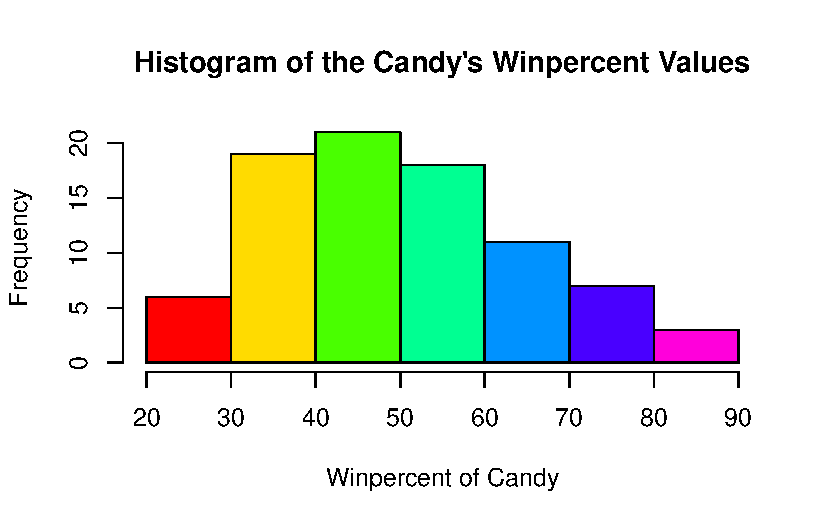
\includegraphics{class10_files/figure-pdf/unnamed-chunk-9-1.pdf}

}

\end{figure}

\emph{Or using ggplot2 packages}

\begin{Shaded}
\begin{Highlighting}[]
\FunctionTok{library}\NormalTok{(ggplot2)}
\FunctionTok{ggplot}\NormalTok{(candy) }\SpecialCharTok{+}
  \FunctionTok{aes}\NormalTok{(winpercent) }\SpecialCharTok{+}
  \FunctionTok{geom\_histogram}\NormalTok{(}\AttributeTok{bins =} \DecValTok{10}\NormalTok{, }\AttributeTok{col =} \StringTok{"red"}\NormalTok{, }\AttributeTok{fill =} \StringTok{"blue"}\NormalTok{) }\SpecialCharTok{+}
  \FunctionTok{labs}\NormalTok{(}\AttributeTok{title =} \StringTok{"Histogram of the Candy\textquotesingle{}s Winpercent Values"}\NormalTok{, }
       \AttributeTok{x =} \StringTok{"Winpercent of Candy"}\NormalTok{, }\AttributeTok{y =} \StringTok{"Frequency"}\NormalTok{)}
\end{Highlighting}
\end{Shaded}

\begin{figure}[H]

{\centering 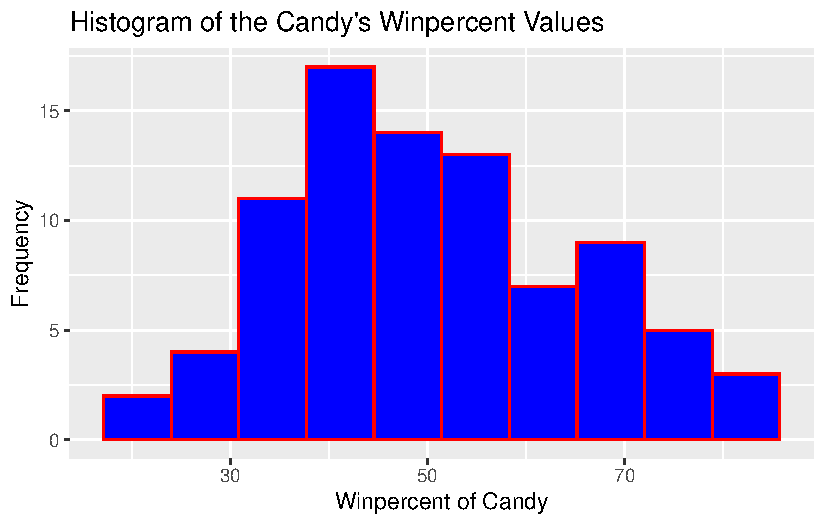
\includegraphics{class10_files/figure-pdf/unnamed-chunk-10-1.pdf}

}

\end{figure}

\begin{quote}
\textbf{Q9. Is the distribution of winpercent values symmetrical?}
\end{quote}

\begin{quote}
\textbf{Ans9: No, the distribution of winpercent values is not
symmetrical.}
\end{quote}

\begin{quote}
\textbf{Q10. Is the center of the distribution above or below 50\%?}
\end{quote}

\begin{quote}
\textbf{Ans10: The center of the distribution is above 50\%}
\end{quote}

\begin{quote}
\textbf{Q11. On average is chocolate candy higher or lower ranked than
fruit candy?}
\end{quote}

\begin{Shaded}
\begin{Highlighting}[]
\NormalTok{chocolate.ind }\OtherTok{\textless{}{-}} \FunctionTok{as.logical}\NormalTok{(candy}\SpecialCharTok{$}\NormalTok{chocolate)}
\FunctionTok{head}\NormalTok{(candy[chocolate.ind,])}
\end{Highlighting}
\end{Shaded}

\begin{verbatim}
                 chocolate fruity caramel peanutyalmondy nougat
100 Grand                1      0       1              0      0
3 Musketeers             1      0       0              0      1
Almond Joy               1      0       0              1      0
Baby Ruth                1      0       1              1      1
Charleston Chew          1      0       0              0      1
HersheyÕs Kisses         1      0       0              0      0
                 crispedricewafer hard bar pluribus sugarpercent pricepercent
100 Grand                       1    0   1        0        0.732        0.860
3 Musketeers                    0    0   1        0        0.604        0.511
Almond Joy                      0    0   1        0        0.465        0.767
Baby Ruth                       0    0   1        0        0.604        0.767
Charleston Chew                 0    0   1        0        0.604        0.511
HersheyÕs Kisses                0    0   0        1        0.127        0.093
                 winpercent
100 Grand          66.97173
3 Musketeers       67.60294
Almond Joy         50.34755
Baby Ruth          56.91455
Charleston Chew    38.97504
HersheyÕs Kisses   55.37545
\end{verbatim}

\begin{Shaded}
\begin{Highlighting}[]
\NormalTok{chocolate.wins }\OtherTok{\textless{}{-}}\NormalTok{ candy[chocolate.ind,]}\SpecialCharTok{$}\NormalTok{winpercent}
\NormalTok{chocolate.wins}
\end{Highlighting}
\end{Shaded}

\begin{verbatim}
 [1] 66.97173 67.60294 50.34755 56.91455 38.97504 55.37545 62.28448 56.49050
 [9] 59.23612 57.21925 76.76860 71.46505 66.57458 55.06407 73.09956 60.80070
[17] 64.35334 47.82975 54.52645 70.73564 66.47068 69.48379 81.86626 84.18029
[25] 73.43499 72.88790 65.71629 34.72200 37.88719 76.67378 59.52925 48.98265
[33] 43.06890 45.73675 49.65350 81.64291 49.52411
\end{verbatim}

\begin{Shaded}
\begin{Highlighting}[]
\FunctionTok{round}\NormalTok{(}\FunctionTok{mean}\NormalTok{(chocolate.wins), }\DecValTok{2}\NormalTok{) }\CommentTok{\# Average winpercent of chocolate candy}
\end{Highlighting}
\end{Shaded}

\begin{verbatim}
[1] 60.92
\end{verbatim}

\begin{Shaded}
\begin{Highlighting}[]
\NormalTok{fruity.ind }\OtherTok{\textless{}{-}} \FunctionTok{as.logical}\NormalTok{(candy}\SpecialCharTok{$}\NormalTok{fruity)}
\NormalTok{fruity.wins }\OtherTok{\textless{}{-}}\NormalTok{ candy[fruity.ind,]}\SpecialCharTok{$}\NormalTok{winpercent}
\FunctionTok{round}\NormalTok{(}\FunctionTok{mean}\NormalTok{(fruity.wins), }\DecValTok{2}\NormalTok{) }\CommentTok{\# Average winpercent of fruity candy}
\end{Highlighting}
\end{Shaded}

\begin{verbatim}
[1] 44.12
\end{verbatim}

\begin{quote}
\textbf{Ans11: On average, the chocolate candy (60.92\%) is HIGHER
ranked than the fruit candy (44.12\%).}
\end{quote}

\begin{quote}
\textbf{Q12. Is this difference statistically significant?}
\end{quote}

\begin{Shaded}
\begin{Highlighting}[]
\FunctionTok{t.test}\NormalTok{(chocolate.wins, fruity.wins)}
\end{Highlighting}
\end{Shaded}

\begin{verbatim}

    Welch Two Sample t-test

data:  chocolate.wins and fruity.wins
t = 6.2582, df = 68.882, p-value = 2.871e-08
alternative hypothesis: true difference in means is not equal to 0
95 percent confidence interval:
 11.44563 22.15795
sample estimates:
mean of x mean of y 
 60.92153  44.11974 
\end{verbatim}

\begin{quote}
\textbf{Ans12: Yes, this is difference statistically significant because
the p-value = 2.871e-08, which is less than 0.05.}
\end{quote}

\hypertarget{overall-candy-ranking}{%
\section{3. Overall Candy Ranking}\label{overall-candy-ranking}}

\begin{quote}
\textbf{Q13. What are the five least liked candy types in this set?}
\end{quote}

\begin{Shaded}
\begin{Highlighting}[]
\FunctionTok{head}\NormalTok{(candy[}\FunctionTok{order}\NormalTok{(candy}\SpecialCharTok{$}\NormalTok{winpercent),], }\AttributeTok{n=}\DecValTok{5}\NormalTok{)}
\end{Highlighting}
\end{Shaded}

\begin{verbatim}
                   chocolate fruity caramel peanutyalmondy nougat
Nik L Nip                  0      1       0              0      0
Boston Baked Beans         0      0       0              1      0
Chiclets                   0      1       0              0      0
Super Bubble               0      1       0              0      0
Jawbusters                 0      1       0              0      0
                   crispedricewafer hard bar pluribus sugarpercent pricepercent
Nik L Nip                         0    0   0        1        0.197        0.976
Boston Baked Beans                0    0   0        1        0.313        0.511
Chiclets                          0    0   0        1        0.046        0.325
Super Bubble                      0    0   0        0        0.162        0.116
Jawbusters                        0    1   0        1        0.093        0.511
                   winpercent
Nik L Nip            22.44534
Boston Baked Beans   23.41782
Chiclets             24.52499
Super Bubble         27.30386
Jawbusters           28.12744
\end{verbatim}

\begin{quote}
\textbf{Q14. What are the top 5 all time favorite candy types out of
this set?}
\end{quote}

\begin{Shaded}
\begin{Highlighting}[]
\FunctionTok{tail}\NormalTok{(candy[}\FunctionTok{order}\NormalTok{(candy}\SpecialCharTok{$}\NormalTok{winpercent),], }\AttributeTok{n=}\DecValTok{5}\NormalTok{)}
\end{Highlighting}
\end{Shaded}

\begin{verbatim}
                          chocolate fruity caramel peanutyalmondy nougat
Snickers                          1      0       1              1      1
Kit Kat                           1      0       0              0      0
Twix                              1      0       1              0      0
ReeseÕs Miniatures                1      0       0              1      0
ReeseÕs Peanut Butter cup         1      0       0              1      0
                          crispedricewafer hard bar pluribus sugarpercent
Snickers                                 0    0   1        0        0.546
Kit Kat                                  1    0   1        0        0.313
Twix                                     1    0   1        0        0.546
ReeseÕs Miniatures                       0    0   0        0        0.034
ReeseÕs Peanut Butter cup                0    0   0        0        0.720
                          pricepercent winpercent
Snickers                         0.651   76.67378
Kit Kat                          0.511   76.76860
Twix                             0.906   81.64291
ReeseÕs Miniatures               0.279   81.86626
ReeseÕs Peanut Butter cup        0.651   84.18029
\end{verbatim}

\begin{quote}
\textbf{Q15. Make a first barplot of candy ranking based on winpercent
values}
\end{quote}

\begin{Shaded}
\begin{Highlighting}[]
\FunctionTok{library}\NormalTok{(ggplot2)}
\FunctionTok{ggplot}\NormalTok{(candy) }\SpecialCharTok{+} 
  \FunctionTok{aes}\NormalTok{(winpercent, }\FunctionTok{rownames}\NormalTok{(candy)) }\SpecialCharTok{+}
  \FunctionTok{geom\_col}\NormalTok{() }\SpecialCharTok{+}
  \FunctionTok{labs}\NormalTok{(}\AttributeTok{title =} \StringTok{"First Barplot of Candy Ranking based on Winpercent Values"}\NormalTok{, }
       \AttributeTok{x =} \StringTok{"Winpercent of Candy"}\NormalTok{, }\AttributeTok{y =} \StringTok{"Name of Candy"}\NormalTok{)}
\end{Highlighting}
\end{Shaded}

\begin{figure}[H]

{\centering 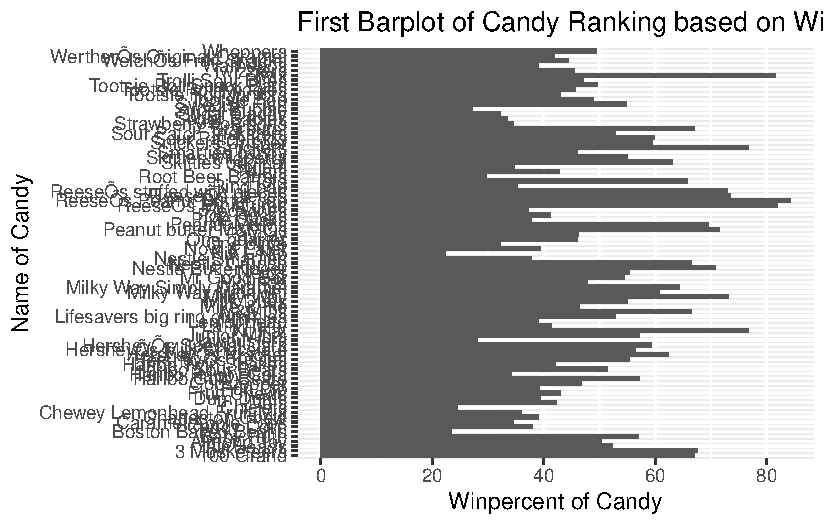
\includegraphics{class10_files/figure-pdf/unnamed-chunk-17-1.pdf}

}

\end{figure}

\begin{quote}
\textbf{Q16. This is quite ugly, use the reorder() function to get the
bars sorted by winpercent?}
\end{quote}

\begin{Shaded}
\begin{Highlighting}[]
\FunctionTok{ggplot}\NormalTok{(candy) }\SpecialCharTok{+} 
  \FunctionTok{aes}\NormalTok{(winpercent, }\FunctionTok{reorder}\NormalTok{(}\FunctionTok{rownames}\NormalTok{(candy),winpercent)) }\SpecialCharTok{+}
  \FunctionTok{geom\_col}\NormalTok{() }\SpecialCharTok{+}
  \FunctionTok{labs}\NormalTok{(}\AttributeTok{title =} \StringTok{"Reorder Barplot of Candy Ranking based on Winpercent Values"}\NormalTok{, }
       \AttributeTok{x =} \StringTok{"Winpercent of Candy"}\NormalTok{, }\AttributeTok{y =} \StringTok{"Name of Candy"}\NormalTok{)}
\end{Highlighting}
\end{Shaded}

\begin{figure}[H]

{\centering 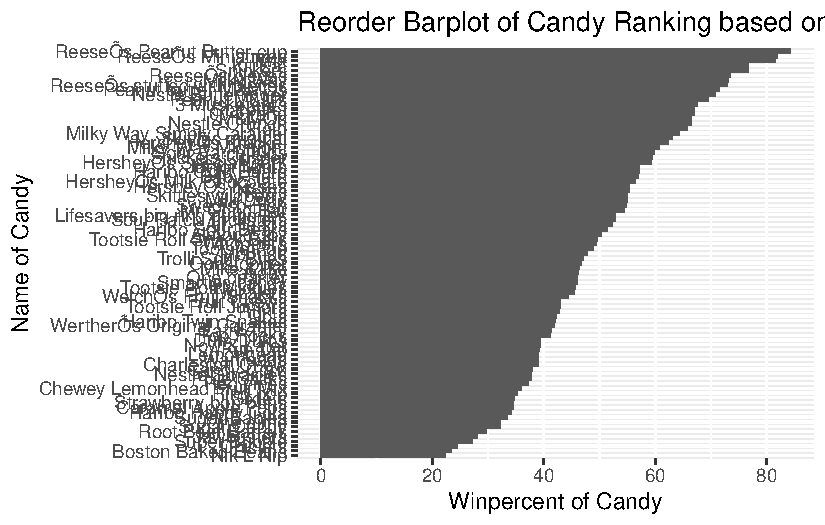
\includegraphics{class10_files/figure-pdf/unnamed-chunk-18-1.pdf}

}

\end{figure}

\hypertarget{time-to-add-some-useful-color}{%
\subsection{Time to add some useful
color}\label{time-to-add-some-useful-color}}

\hypertarget{setup-a-color-vector}{%
\subsubsection{\texorpdfstring{\emph{Setup a color
vector}}{Setup a color vector}}\label{setup-a-color-vector}}

\begin{Shaded}
\begin{Highlighting}[]
\NormalTok{my\_cols}\OtherTok{=}\FunctionTok{rep}\NormalTok{(}\StringTok{"black"}\NormalTok{, }\FunctionTok{nrow}\NormalTok{(candy))}
\NormalTok{my\_cols[}\FunctionTok{as.logical}\NormalTok{(candy}\SpecialCharTok{$}\NormalTok{chocolate)] }\OtherTok{=} \StringTok{"chocolate"}
\NormalTok{my\_cols[}\FunctionTok{as.logical}\NormalTok{(candy}\SpecialCharTok{$}\NormalTok{bar)] }\OtherTok{=} \StringTok{"red"}
\NormalTok{my\_cols[}\FunctionTok{as.logical}\NormalTok{(candy}\SpecialCharTok{$}\NormalTok{fruity)] }\OtherTok{=} \StringTok{"green"}
\end{Highlighting}
\end{Shaded}

\hypertarget{try-improve-barplot-with-these-colors}{%
\subsubsection{\texorpdfstring{\emph{Try improve barplot with these
colors}}{Try improve barplot with these colors}}\label{try-improve-barplot-with-these-colors}}

\begin{Shaded}
\begin{Highlighting}[]
\FunctionTok{ggplot}\NormalTok{(candy) }\SpecialCharTok{+} 
  \FunctionTok{aes}\NormalTok{(winpercent, }\FunctionTok{reorder}\NormalTok{(}\FunctionTok{rownames}\NormalTok{(candy),winpercent)) }\SpecialCharTok{+}
  \FunctionTok{geom\_col}\NormalTok{(}\AttributeTok{fill =}\NormalTok{ my\_cols) }\SpecialCharTok{+}
  \FunctionTok{labs}\NormalTok{(}\AttributeTok{title =} \StringTok{"Barplot of Candy Ranking based on Winpercent Values"}\NormalTok{, }
       \AttributeTok{x =} \StringTok{"Winpercent of Candy"}\NormalTok{, }\AttributeTok{y =} \StringTok{"Name of Candy"}\NormalTok{)}
\end{Highlighting}
\end{Shaded}

\begin{figure}[H]

{\centering 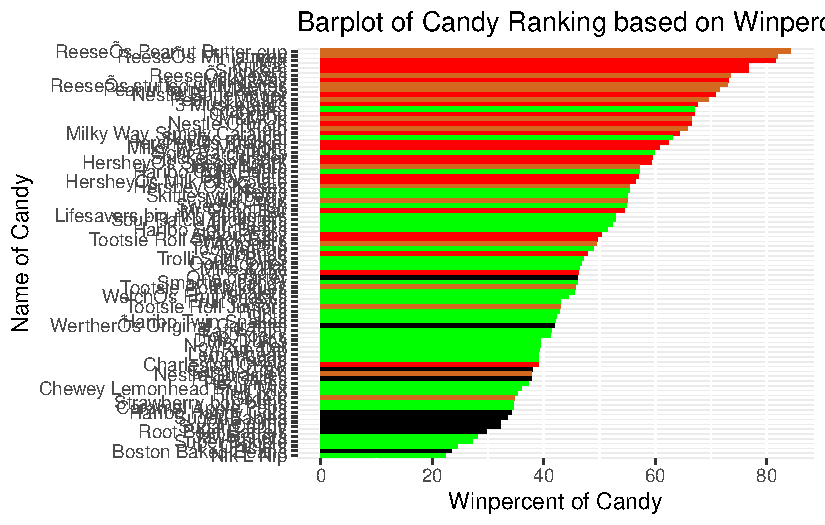
\includegraphics{class10_files/figure-pdf/unnamed-chunk-20-1.pdf}

}

\end{figure}

\begin{Shaded}
\begin{Highlighting}[]
\FunctionTok{ggsave}\NormalTok{(}\StringTok{"tmp.png"}\NormalTok{) }\CommentTok{\# To take a picture of the graph above}
\end{Highlighting}
\end{Shaded}

\begin{verbatim}
Saving 5.5 x 3.5 in image
\end{verbatim}

\begin{quote}
\textbf{Q17. What is the worst ranked chocolate candy?}
\end{quote}

\begin{quote}
\textbf{Ans17: Sixlets}
\end{quote}

\begin{quote}
\textbf{Q18. What is the best ranked fruity candy?}
\end{quote}

\begin{quote}
\textbf{Ans18: Starburst}
\end{quote}

\hypertarget{taking-a-look-at-pricepercent}{%
\section{4. Taking a look at
pricepercent}\label{taking-a-look-at-pricepercent}}

\emph{Note: Install the ``ggrepel'' package first by using
`install.packages(``ggrepel'')' function}

\begin{Shaded}
\begin{Highlighting}[]
\FunctionTok{library}\NormalTok{(ggrepel)}
\CommentTok{\# How about a plot of price vs win}
\FunctionTok{ggplot}\NormalTok{(candy) }\SpecialCharTok{+}
  \FunctionTok{aes}\NormalTok{(winpercent, pricepercent, }\AttributeTok{label =} \FunctionTok{rownames}\NormalTok{(candy)) }\SpecialCharTok{+}
  \FunctionTok{geom\_point}\NormalTok{(}\AttributeTok{col =}\NormalTok{ my\_cols) }\SpecialCharTok{+} 
  \FunctionTok{geom\_text\_repel}\NormalTok{(}\AttributeTok{col =}\NormalTok{ my\_cols, }\AttributeTok{size =} \DecValTok{3}\NormalTok{, }\AttributeTok{max.overlaps =} \DecValTok{9}\NormalTok{) }\SpecialCharTok{+}
  \FunctionTok{labs}\NormalTok{(}\AttributeTok{title =} \StringTok{"Plot of Pricepercent versus Winpercent"}\NormalTok{, }
       \AttributeTok{x =} \StringTok{"Winpercent of Candy"}\NormalTok{, }\AttributeTok{y =} \StringTok{"Pricepercent of Candy"}\NormalTok{)}
\end{Highlighting}
\end{Shaded}

\begin{verbatim}
Warning: ggrepel: 52 unlabeled data points (too many overlaps). Consider
increasing max.overlaps
\end{verbatim}

\begin{figure}[H]

{\centering 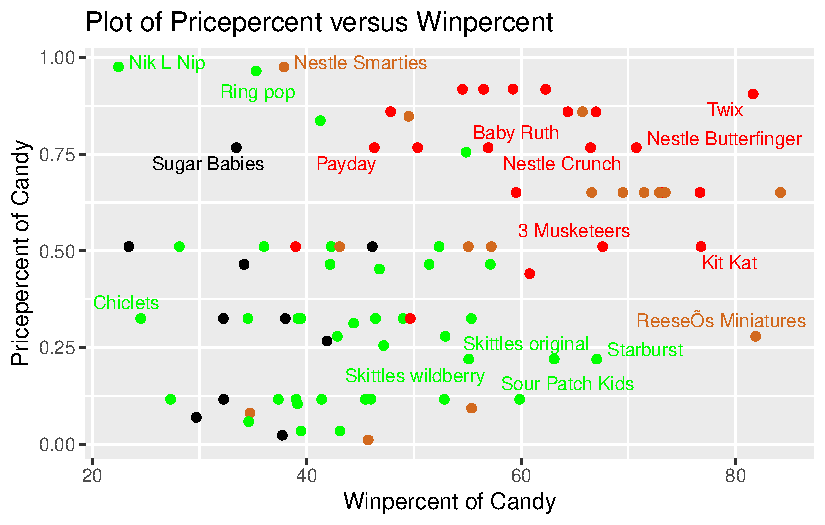
\includegraphics{class10_files/figure-pdf/unnamed-chunk-22-1.pdf}

}

\end{figure}

\begin{quote}
\textbf{Q19. Which candy type is the highest ranked in terms of
winpercent for the least money - i.e.~offers the most bang for your
buck?}
\end{quote}

\begin{quote}
\textbf{Ans19: Fruity candy type}
\end{quote}

\begin{quote}
\textbf{Q20. What are the top 5 most expensive candy types in the
dataset and of these which is the least popular?}
\end{quote}

\begin{Shaded}
\begin{Highlighting}[]
\NormalTok{ord }\OtherTok{\textless{}{-}} \FunctionTok{order}\NormalTok{(candy}\SpecialCharTok{$}\NormalTok{pricepercent, }\AttributeTok{decreasing =} \ConstantTok{TRUE}\NormalTok{)}
\FunctionTok{head}\NormalTok{( candy[ord,}\FunctionTok{c}\NormalTok{(}\DecValTok{11}\NormalTok{,}\DecValTok{12}\NormalTok{)], }\AttributeTok{n=}\DecValTok{5}\NormalTok{ )}
\end{Highlighting}
\end{Shaded}

\begin{verbatim}
                         pricepercent winpercent
Nik L Nip                       0.976   22.44534
Nestle Smarties                 0.976   37.88719
Ring pop                        0.965   35.29076
HersheyÕs Krackel               0.918   62.28448
HersheyÕs Milk Chocolate        0.918   56.49050
\end{verbatim}

\hypertarget{optional}{%
\subsection{Optional}\label{optional}}

\begin{quote}
\textbf{Q21. Make a barplot again with geom\_col() this time using
pricepercent and then improve this step by step, first ordering the
x-axis by value and finally making a so called ``dot chat'' or
``lollipop'' chart by swapping geom\_col() for geom\_point() +
geom\_segment().}
\end{quote}

\begin{Shaded}
\begin{Highlighting}[]
\FunctionTok{ggplot}\NormalTok{(candy) }\SpecialCharTok{+} 
  \FunctionTok{aes}\NormalTok{(pricepercent, }\FunctionTok{reorder}\NormalTok{(}\FunctionTok{rownames}\NormalTok{(candy),pricepercent)) }\SpecialCharTok{+}
  \FunctionTok{geom\_col}\NormalTok{() }\SpecialCharTok{+}
  \FunctionTok{labs}\NormalTok{(}\AttributeTok{title =} \StringTok{"Barplot of Candy Ranking based on Pricepercent Values"}\NormalTok{, }
       \AttributeTok{x =} \StringTok{"Pricepercent of Candy"}\NormalTok{, }\AttributeTok{y =} \StringTok{"Name of Candy"}\NormalTok{)}
\end{Highlighting}
\end{Shaded}

\begin{figure}[H]

{\centering 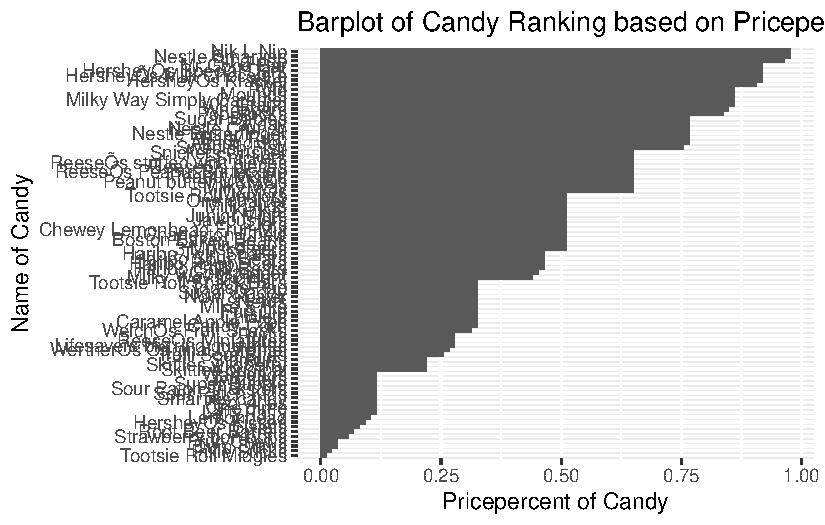
\includegraphics{class10_files/figure-pdf/unnamed-chunk-24-1.pdf}

}

\end{figure}

\begin{Shaded}
\begin{Highlighting}[]
\CommentTok{\# Make a lollipop chart of pricepercent}
\FunctionTok{ggplot}\NormalTok{(candy) }\SpecialCharTok{+}
  \FunctionTok{aes}\NormalTok{(pricepercent, }\FunctionTok{reorder}\NormalTok{(}\FunctionTok{rownames}\NormalTok{(candy), pricepercent)) }\SpecialCharTok{+}
  \FunctionTok{geom\_segment}\NormalTok{(}\FunctionTok{aes}\NormalTok{(}\AttributeTok{yend =} \FunctionTok{reorder}\NormalTok{(}\FunctionTok{rownames}\NormalTok{(candy), pricepercent), }
                   \AttributeTok{xend =} \DecValTok{0}\NormalTok{), }\AttributeTok{col=}\StringTok{"gray40"}\NormalTok{) }\SpecialCharTok{+}
  \FunctionTok{geom\_point}\NormalTok{() }\SpecialCharTok{+}
  \FunctionTok{labs}\NormalTok{(}\AttributeTok{title =} \StringTok{"Lollipop Chart of Candy Ranking based on Pricepercent Values"}\NormalTok{, }
       \AttributeTok{x =} \StringTok{"Pricepercent of Candy"}\NormalTok{, }\AttributeTok{y =} \StringTok{"Name of Candy"}\NormalTok{)}
\end{Highlighting}
\end{Shaded}

\begin{figure}[H]

{\centering 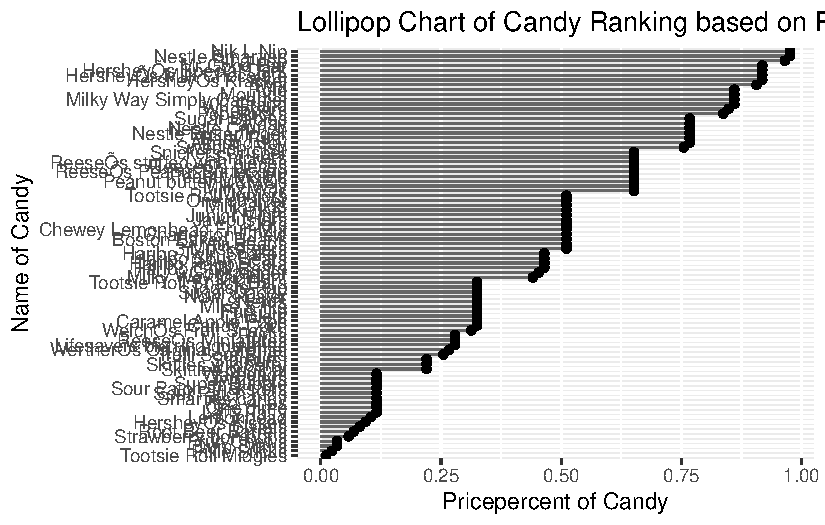
\includegraphics{class10_files/figure-pdf/unnamed-chunk-25-1.pdf}

}

\end{figure}

\hypertarget{exploring-the-correlation-structure}{%
\section{5 Exploring the correlation
structure}\label{exploring-the-correlation-structure}}

\emph{Note: Install the ``corrplot'' package first by using
`install.packages(``corrplot'')' function}

\begin{Shaded}
\begin{Highlighting}[]
\FunctionTok{library}\NormalTok{(corrplot)}
\end{Highlighting}
\end{Shaded}

\begin{verbatim}
corrplot 0.92 loaded
\end{verbatim}

\begin{Shaded}
\begin{Highlighting}[]
\NormalTok{cij }\OtherTok{\textless{}{-}} \FunctionTok{cor}\NormalTok{(candy)}
\FunctionTok{corrplot}\NormalTok{(cij)}
\end{Highlighting}
\end{Shaded}

\begin{figure}[H]

{\centering 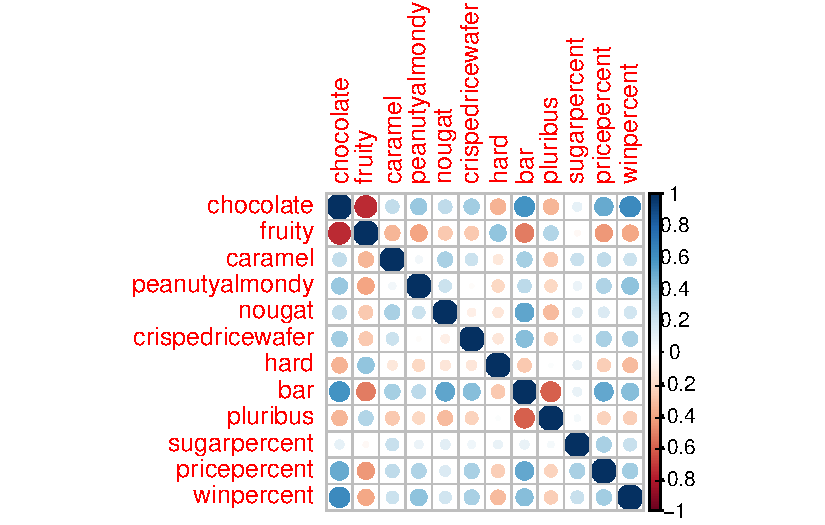
\includegraphics{class10_files/figure-pdf/unnamed-chunk-27-1.pdf}

}

\end{figure}

\begin{quote}
\textbf{Q22. Examining this plot what two variables are anti-correlated
(i.e.~have minus values)?}
\end{quote}

\begin{quote}
\textbf{Ans22: Chocolate and Fruity are anti-correlated.}
\end{quote}

\begin{quote}
\textbf{Q23. Similarly, what two variables are most positively
correlated?}
\end{quote}

\begin{quote}
\textbf{Ans23: Chocolate and Bar (or Chocolate and Winpercent) are most
positively correlated}
\end{quote}

\hypertarget{principal-component-analysis}{%
\section{6. Principal Component
Analysis}\label{principal-component-analysis}}

\begin{Shaded}
\begin{Highlighting}[]
\NormalTok{pca }\OtherTok{\textless{}{-}} \FunctionTok{prcomp}\NormalTok{(candy, }\AttributeTok{scale =} \ConstantTok{TRUE}\NormalTok{)}
\FunctionTok{summary}\NormalTok{(pca)}
\end{Highlighting}
\end{Shaded}

\begin{verbatim}
Importance of components:
                          PC1    PC2    PC3     PC4    PC5     PC6     PC7
Standard deviation     2.0788 1.1378 1.1092 1.07533 0.9518 0.81923 0.81530
Proportion of Variance 0.3601 0.1079 0.1025 0.09636 0.0755 0.05593 0.05539
Cumulative Proportion  0.3601 0.4680 0.5705 0.66688 0.7424 0.79830 0.85369
                           PC8     PC9    PC10    PC11    PC12
Standard deviation     0.74530 0.67824 0.62349 0.43974 0.39760
Proportion of Variance 0.04629 0.03833 0.03239 0.01611 0.01317
Cumulative Proportion  0.89998 0.93832 0.97071 0.98683 1.00000
\end{verbatim}

\begin{Shaded}
\begin{Highlighting}[]
\FunctionTok{plot}\NormalTok{(pca}\SpecialCharTok{$}\NormalTok{x[,}\DecValTok{1}\NormalTok{], pca}\SpecialCharTok{$}\NormalTok{x[,}\DecValTok{2}\NormalTok{], }
     \AttributeTok{main =} \StringTok{"PC1 and PC2 Plot"}\NormalTok{, }\AttributeTok{xlab =} \StringTok{"PC1"}\NormalTok{, }\AttributeTok{ylab =} \StringTok{"PC2"}\NormalTok{)}
\end{Highlighting}
\end{Shaded}

\begin{figure}[H]

{\centering 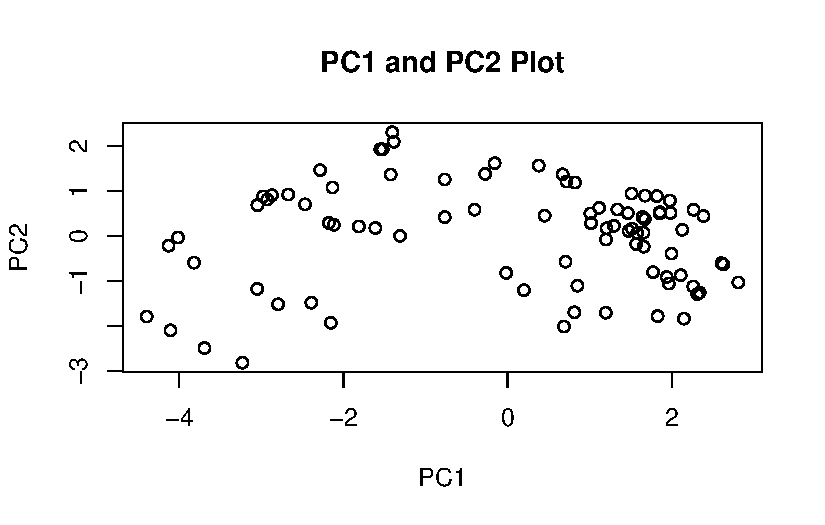
\includegraphics{class10_files/figure-pdf/unnamed-chunk-29-1.pdf}

}

\end{figure}

\begin{Shaded}
\begin{Highlighting}[]
\FunctionTok{plot}\NormalTok{(pca}\SpecialCharTok{$}\NormalTok{x[,}\DecValTok{1}\SpecialCharTok{:}\DecValTok{2}\NormalTok{], }\AttributeTok{col =}\NormalTok{ my\_cols, }\AttributeTok{pch =} \DecValTok{15}\NormalTok{, }
     \AttributeTok{main =} \StringTok{"PC1 and PC2 Plot"}\NormalTok{, }\AttributeTok{xlab =} \StringTok{"PC1"}\NormalTok{, }\AttributeTok{ylab =} \StringTok{"PC2"}\NormalTok{)}
\end{Highlighting}
\end{Shaded}

\begin{figure}[H]

{\centering 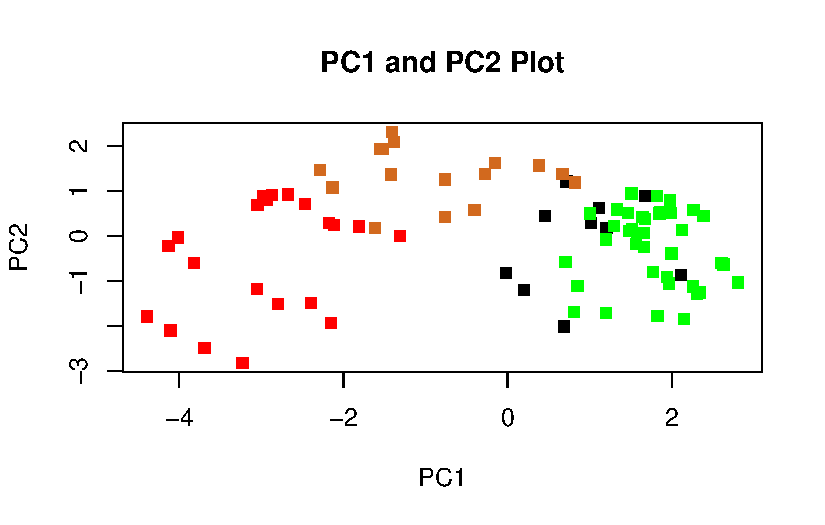
\includegraphics{class10_files/figure-pdf/unnamed-chunk-30-1.pdf}

}

\end{figure}

\begin{Shaded}
\begin{Highlighting}[]
\CommentTok{\# Make a new data{-}frame with our PCA results and candy data}
\NormalTok{my\_data }\OtherTok{\textless{}{-}} \FunctionTok{cbind}\NormalTok{(candy, pca}\SpecialCharTok{$}\NormalTok{x[,}\DecValTok{1}\SpecialCharTok{:}\DecValTok{3}\NormalTok{])}
\end{Highlighting}
\end{Shaded}

\begin{Shaded}
\begin{Highlighting}[]
\NormalTok{p }\OtherTok{\textless{}{-}} \FunctionTok{ggplot}\NormalTok{(my\_data) }\SpecialCharTok{+} 
        \FunctionTok{aes}\NormalTok{(}\AttributeTok{x=}\NormalTok{PC1, }\AttributeTok{y=}\NormalTok{PC2, }
            \AttributeTok{size=}\NormalTok{winpercent}\SpecialCharTok{/}\DecValTok{100}\NormalTok{,  }
            \AttributeTok{text=}\FunctionTok{rownames}\NormalTok{(my\_data),}
            \AttributeTok{label=}\FunctionTok{rownames}\NormalTok{(my\_data)) }\SpecialCharTok{+}
        \FunctionTok{geom\_point}\NormalTok{(}\AttributeTok{col=}\NormalTok{my\_cols)}

\NormalTok{p}
\end{Highlighting}
\end{Shaded}

\begin{figure}[H]

{\centering 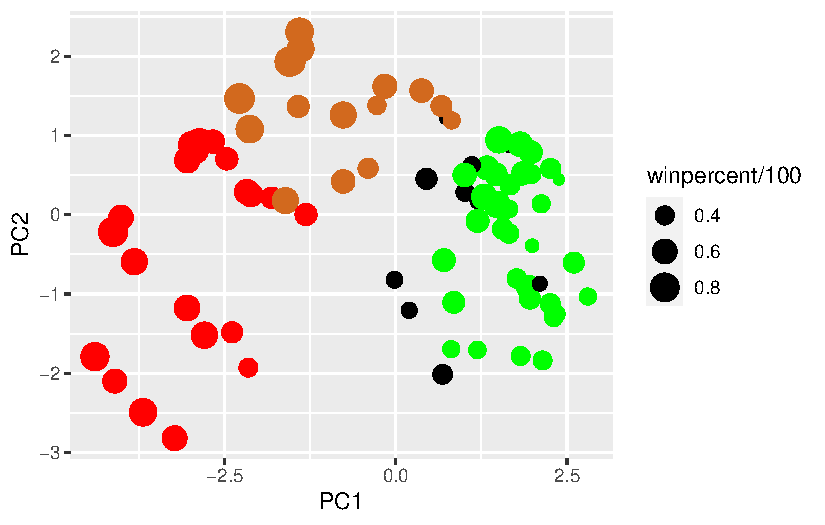
\includegraphics{class10_files/figure-pdf/unnamed-chunk-32-1.pdf}

}

\end{figure}

\begin{Shaded}
\begin{Highlighting}[]
\FunctionTok{library}\NormalTok{(ggrepel)}

\NormalTok{p }\SpecialCharTok{+} \FunctionTok{geom\_text\_repel}\NormalTok{(}\AttributeTok{size =} \DecValTok{3}\NormalTok{, }\AttributeTok{col=}\NormalTok{my\_cols, }\AttributeTok{max.overlaps =} \DecValTok{9}\NormalTok{)  }\SpecialCharTok{+} 
  \FunctionTok{theme}\NormalTok{(}\AttributeTok{legend.position =} \StringTok{"none"}\NormalTok{) }\SpecialCharTok{+}
  \FunctionTok{labs}\NormalTok{(}\AttributeTok{title =} \StringTok{"Halloween Candy PCA Space"}\NormalTok{,}
       \AttributeTok{subtitle =} \StringTok{"Colored by type: chocolate bar (red),}
\StringTok{       chocolate other (light brown),}
\StringTok{       fruity (light green),}
\StringTok{       other (black)"}\NormalTok{,}
       \AttributeTok{caption =} \StringTok{"Data from FiveThirtyEight (538)"}\NormalTok{)}
\end{Highlighting}
\end{Shaded}

\begin{verbatim}
Warning: ggrepel: 60 unlabeled data points (too many overlaps). Consider
increasing max.overlaps
\end{verbatim}

\begin{figure}[H]

{\centering 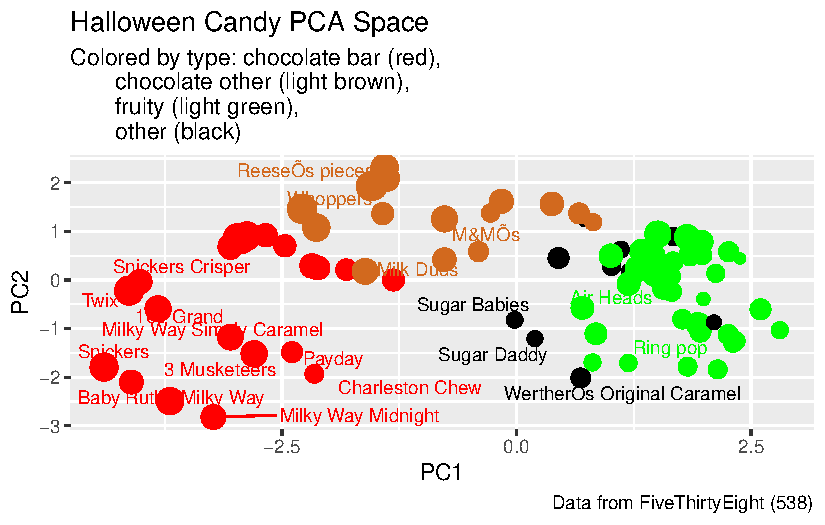
\includegraphics{class10_files/figure-pdf/unnamed-chunk-33-1.pdf}

}

\end{figure}

\emph{Note: Install ``plotly'' package first by using
`install.packages(``plotly'')' function}

\begin{Shaded}
\begin{Highlighting}[]
\FunctionTok{library}\NormalTok{(plotly)}
\end{Highlighting}
\end{Shaded}

\begin{verbatim}

Attaching package: 'plotly'
\end{verbatim}

\begin{verbatim}
The following object is masked from 'package:ggplot2':

    last_plot
\end{verbatim}

\begin{verbatim}
The following object is masked from 'package:stats':

    filter
\end{verbatim}

\begin{verbatim}
The following object is masked from 'package:graphics':

    layout
\end{verbatim}

\begin{Shaded}
\begin{Highlighting}[]
\FunctionTok{ggplotly}\NormalTok{(p)}
\end{Highlighting}
\end{Shaded}

\begin{Shaded}
\begin{Highlighting}[]
\FunctionTok{par}\NormalTok{(}\AttributeTok{mar=}\FunctionTok{c}\NormalTok{(}\DecValTok{8}\NormalTok{,}\DecValTok{4}\NormalTok{,}\DecValTok{2}\NormalTok{,}\DecValTok{2}\NormalTok{))}
\FunctionTok{barplot}\NormalTok{(pca}\SpecialCharTok{$}\NormalTok{rotation[,}\DecValTok{1}\NormalTok{], }\AttributeTok{las=}\DecValTok{2}\NormalTok{, }\AttributeTok{ylab=}\StringTok{"PC1 Contribution"}\NormalTok{, }\AttributeTok{col =} \FunctionTok{rainbow}\NormalTok{(}\DecValTok{12}\NormalTok{))}
\end{Highlighting}
\end{Shaded}

\begin{figure}[H]

{\centering 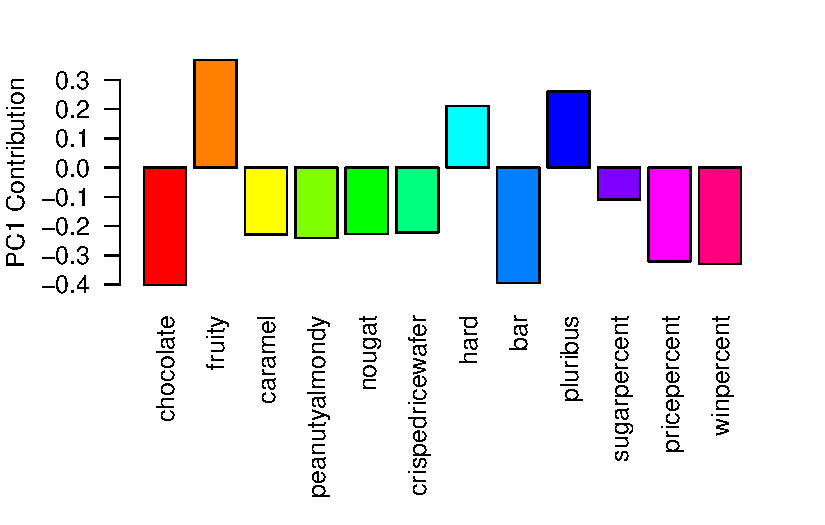
\includegraphics{class10_files/figure-pdf/unnamed-chunk-36-1.pdf}

}

\end{figure}

\begin{quote}
\textbf{Q24. What original variables are picked up strongly by PC1 in
the positive direction? Do these make sense to you?}
\end{quote}

\begin{quote}
\textbf{Ans24: Fruity, Hard, and Pluribus are picked up strongly by PC1
in the positive direction. These make sense since they are positive
correlations, fruity candies are usually hard, and they are usually set
in a bag or a box of multiple fruity candy flavors.}
\end{quote}



\end{document}
